% !TeX TXS-program:compile = txs:///lualatex/[--shell-escape]

%----------------------- Преамбула -----------------------
\documentclass[ut8x, 14pt, oneside, a4paper]{extarticle}

\usepackage{extsizes} % Для добавления в параметры класса документа 14pt

% Для работы с несколькими языками и шрифтом Times New Roman по-умолчанию
\usepackage[english,russian]{babel}
\usepackage{fontspec}
\setmainfont{Times New Roman}
\usepackage[left=30mm,right=10mm,top=20mm,bottom=20mm]{geometry}
\usepackage{misccorr}
\usepackage{indentfirst}
\usepackage{enumitem}
\usepackage{pdfpages}
%\usepackage{ragged2e}
\setlength{\parindent}{1.25cm}
%\setlength{\parskip}{1em} % поменять
%\linespread{1.3}
\renewcommand{\baselinestretch}{1.5}
\setlist{nolistsep} % Отсутствие отступов между элементами \enumerate и \itemize

% Дополнительное окружения для подписей
\usepackage{array}
\newenvironment{signstabular}[1][1]{
	\renewcommand*{\arraystretch}{#1}
	\tabular
}{
	\endtabular
}

% Переопределение стандартных \section, \subsection, \subsubsection по ГОСТу;
% Переопределение их отступов до и после для 1.5 интервала во всем документе
\usepackage{titlesec}

\titleformat{\section}[block]
{\bfseries\normalsize\filcenter}{\thesection}{1em}{}

\titleformat{\subsection}[hang]
{\bfseries\normalsize}{\thesubsection}{1em}{}
\titlespacing\subsection{\parindent}{\parskip}{\parskip}

\titleformat{\subsubsection}[hang]
{\bfseries\normalsize}{\thesubsubsection}{1em}{}
\titlespacing\subsubsection{\parindent}{\parskip}{\parskip}

\newcommand{\specsection}[1]{\section*{#1}\addcontentsline{toc}{section}{#1}}

% Работа с изображениями и таблицами; переопределение названий по ГОСТу
\usepackage{caption}
\captionsetup[figure]{name={Рисунок},labelsep=endash}
\captionsetup[table]{singlelinecheck=false, labelsep=endash}

\usepackage{graphicx}
\usepackage{diagbox} % Диагональное разделение первой ячейки в таблицах

% Цвета для гиперссылок и листингов
\usepackage{color}

% Гиперссылки \toc с кликабельностью
\usepackage[linktoc=all]{hyperref}
\hypersetup{hidelinks}

% Листинги
%\setsansfont{Arial}
%\setmonofont{Courier New}

\usepackage{color} % Цвета для гиперссылок и листингов
%\definecolor{comment}{rgb}{0,0.5,0}
%\definecolor{plain}{rgb}{0.2,0.2,0.2}
%\definecolor{string}{rgb}{0.91,0.45,0.32}
%\hypersetup{citecolor=blue}
\hypersetup{citecolor=black}

\usepackage{listings}
\lstset{
	basicstyle=\footnotesize\ttfamily,
	language=XML,
	numbers=left,
	numbersep=5pt,
	tabsize=2,
	extendedchars=\true,
	breaklines=true,
	keywordstyle=\color{blue},
	frame=single,
	showspaces=false,
	showtabs=false,
	xleftmargin=17pt,
	framexleftmargin=17pt,
	framexrightmargin=-5pt,
	framexbottommargin=4pt,
	showstringspaces=false,
	inputencoding=utf8x,
	keepspaces=true
}

\usepackage{ulem} % Нормальное нижнее подчеркивание
\usepackage{hhline} % Двойная горизонтальная линия в таблицах
\usepackage[figure,table]{totalcount} % Подсчет изображений, таблиц
\usepackage{rotating} % Поворот изображения вместе с названием
\usepackage{lastpage} % Для подсчета числа страниц

\makeatletter
\renewcommand\@biblabel[1]{#1.}
\makeatother

\usepackage{color}
\usepackage[cache=false, newfloat]{minted}
\newenvironment{code}{\captionsetup{type=listing}}{}
\SetupFloatingEnvironment{listing}{name=Листинг}

\usepackage{amsmath}
\usepackage{slashbox}


\begin{document}
	
\begin{titlepage}
	\noindent\begin{minipage}{0.05\textwidth}
		
\includegraphics[scale=0.3]{inc/bmstu.png}
	\end{minipage}
	\hfill
	\begin{minipage}{0.85\textwidth}\raggedleft
		\begin{center}
			\fontsize{12pt}{0.3\baselineskip}\selectfont \textbf{Министерство науки и высшего образования Российской Федерации \\ Федеральное государственное бюджетное образовательное учреждение \\ высшего образования \\ <<Московский государственный технический университет \\ имени Н.Э. Баумана \\ (национальный исследовательский университет)>> \\ (МГТУ им. Н.Э. Баумана)}
		\end{center}
	\end{minipage}

	\begin{center}
		\fontsize{12pt}{0.1\baselineskip}\selectfont
		\noindent\makebox[\linewidth]{\rule{\textwidth}{4pt}} \makebox[\linewidth]{\rule{\textwidth}{1pt}}
	\end{center}

	\begin{flushleft}
		\fontsize{12pt}{0.8\baselineskip}\selectfont 
		
		ФАКУЛЬТЕТ \uline{<<\textbf{Информатика и системы управления}>> \hfill}

		КАФЕДРА \uline{\mbox{\hspace{4mm}} <<\textbf{Программное обеспечение ЭВМ и информационные технологии}>> \hfill}
	\end{flushleft}

	\vfill

	\begin{center}
		\fontsize{20pt}{\baselineskip}\selectfont

		\uline{\textbf{ОТЧЁТ ПО ПРОИЗВОДСТВЕННОЙ ПРАКТИКЕ}}
	\end{center}
	
	\vfill
	
	\begin{flushleft}
		\fontsize{12pt}{0.7\baselineskip}\selectfont

		Студент \uline{\mbox{\hspace{44mm}} Романов Семен Константинович \hfill}
		
		Группа \uline{\mbox{\hspace{64mm}} ИУ7-65Б \hfill}
		
		Тип практики \uline{\mbox{\hspace{44mm}} Производственная \hfill}
		
		Название предприятия \uline{\mbox{\hspace{26mm}} ООО~<<СитиСофт>> \hfill}
	\end{flushleft}	

	\vfill

	\begin{table}[h!]
		\fontsize{12pt}{0.7\baselineskip}\selectfont

		\begin{signstabular}[0.55]{p{7.25cm} >{\centering\arraybackslash}p{4cm} >{\centering\arraybackslash}p{4cm}}
		Студент & \uline{\mbox{\hspace*{4cm}}} & \uline{\hfill \textbf{Романов С. К.} \hfill} \\
		& \scriptsize \textit{подпись, дата} & \scriptsize \textit{фамилия, и.о.}
		\end{signstabular}
	
		\vspace{\baselineskip}

		\begin{signstabular}[0.55]{p{7.25cm} >{\centering\arraybackslash}p{4cm} >{\centering\arraybackslash}p{4cm}}
			Руководитель практики & \uline{\mbox{\hspace*{4cm}}} & \uline{\hfill \textbf{Толпинская Н. Б.} \hfill} \\
			\mbox{\hspace*{1cm}} \scriptsize (от университета) & \scriptsize \textit{подпись, дата} & \scriptsize \textit{фамилия, и.о.}
		\end{signstabular}

		\vspace{\baselineskip}
		
		\begin{signstabular}[0.55]{p{7.25cm} >{\centering\arraybackslash}p{4cm} >{\centering\arraybackslash}p{4cm}}
			Руководитель практики & \uline{\mbox{\hspace*{4cm}}} & \uline{\hfill \textbf{Батин Р. Е.} \hfill} \\
			\mbox{\hspace*{1cm}} \scriptsize (от предприятия) & \scriptsize \textit{подпись, дата} & \scriptsize \textit{фамилия, и.о.}
		\end{signstabular}
	
		\vspace{\baselineskip}
		
		\begin{signstabular}[0.55]{p{7.25cm} >{\centering\arraybackslash}p{4cm} >{\centering\arraybackslash}p{4cm}}
			Оценка~~\uline{\hfill}
		\end{signstabular} 
	 
	\end{table}

	\vfill

	\begin{center}
		\normalsize \textit{\the\year~г.}
	\end{center}
\end{titlepage}

\normalsize

\pagenumbering{arabic}
\setcounter{page}{2}

\tableofcontents
\normalsize

\pagebreak

\specsection{ВВЕДЕНИЕ}

\texttt{BOB} --- это распределённая система хранения данных типа ключ-значение~\cite{BOB}. \texttt{BOB} проектировался для быстрой и надёжной работы с бинарными данными средних размеров (например, с изображениями). \texttt{BOB} постоянно развивается и обладает множеством запланированных задач разной сложности.

Цель производственной практики --- овладеть навыками разработки систем хранения данных, Web-приложений~\cite{web}, open source-проектов~\cite{oss} 

Задачи проекта:

Разработать Web-приложение~\cite{web}, включающее в себя:
\begin{enumerate}
	\item страницу авторизации;
	\item домашнюю страницу с основными параметрами кластера;
	\item страницу с нодами;
	\item страницу с подробной информацией о ноде;
	\item страницу с раскладкой виртуальных дисков.
\end{enumerate}

Индивидуальные задачи: 

\begin{enumerate}
	\item получить навыки командной работы;
	\item спроектировать и разработать клиент для взаимодействия с API~\cite{api} Боба;
	\item спроектировать собственный API~\cite{api};
	\item разработать серверную часть веб-приложения, интегрируя в него ранее разработанный клиент и API~\cite{api};
	\item провести тестирование итогового Web-приложения.
\end{enumerate}

\clearpage

\section{Характеристика предприятия}

Компания <<СитиСофт>> предоставляет высококачественные услуги для тех, кто стремится улучшить свой бизнес путем внедрения или обновления программно - аппаратной инфраструктуры.

Продукты <<СитиСофт>> --- это специальные технические средства и комплексы, серверы и компьютерные компоненты, активное и пассивное сетевое оборудование, Системы Хранения Данных и специализированное ПО, а так же решения на базе оборудования ведущих мировых производителей и многое другое.

Предлагаемые услуги включает самые востребованные на сегодняшний день IT-проекты, позволяющие масштабировать решения, получить максимальный технологический эффект. 

Это построение специальных систем различного уровня, создание систем обработки и хранения данных, централизация и виртуализация IT-сервиса, информационная защита и резервное копирование, решения по видеонаблюдению, IP-телефонии и многое другое~\cite{citysoft}.

\clearpage

\section{Характеристика проекта для производственной практики}

Требуется разработать Web-приложение, включающее в себя следующее: 

\begin{enumerate}
  \item[$-$] Страница авторизации. На странице необходимо задавать адрес входной ноды и опционально логин и пароль.
  \item[$-$] Домашняя страница с основными параметрами кластера: число нод в кластере, число рабочих нод, число нод с проблемами, число нерабочих нод, информация по физическим дискам аналогична. Также необходимо включить общее число обрабатываемых запросов на кластере в секунду с разбивкой далее по put, get, exist, delete, общее место на дисках кластера, занятое данными место на дисках всего кластера. 
  \item[$-$] Страница с нодами. Страница должна отображать все ноды с именем и адресом, по каждой ноде её состояние -- работает, есть проблемы, не работает; операции в секунду на ноде; занятое дисковое пространство. Перечень проблем на ноде: не доступен один из дисков, есть alien’ы, есть поврежденные БЛОБы, осталось свободного места менее 10\%, виртуальная память, выделенная ноде, превышает доступную физическую память, нагрузка на CPU выше 90\%. С данной страницы должна быть реализована возможность перехода на страницу с подробной информации о ноде.
  \item[$-$] Страница с подробной информацией о ноде. Страница должна демонстрировать основные метрики ноды, параметры системы, на которой запущена нода -- загрузка CPU, RAM, дескрипторы; список дисков на ноде с их состоянием, список виртуальных дисков внутри каждого диска. Также дать возможность просмотра целиком метрик ноды в виде таблицы.
  \item[$-$] Страница с раскладкой виртуальных дисков. Страница должна отображать список виртуальных дисков с их доступностью в кластере.
\end{enumerate}

\clearpage

\section{Характеристика индивидуального задания для производственной практики}

В ходе практики предстоит выполнить следующие индивидуальные задачи:
\begin{enumerate}[label={\arabic*.}]
  \item Студент должен овладеть навыками командной работы, что позволит ему эффективно сотрудничать с другими разработчиками в рамках проекта.
  \item Спроектировать и разработать клиент для взаимодействия с API~\cite{api} \texttt{BOB}. Данную задачу необходимо реализовать в первую очередь, поскольку клиент будет обеспечивать сервер данными о распределенной системе хранения данных.
  \item Спроектировать собственный API~\cite{api}, который позволит серверной части Web-приложения~\cite{web} передавать данные внешнему интефейсу. Это API должно быть хорошо продумано, чтобы обеспечить удобный и эффективный доступ к данным \texttt{BOB}'a.
  \item Разработать серверную часть Web-приложения~\cite{web}, включив в него ранее разработанный клиент и API. Это будет являться основной частью работы, так как сервер должен обеспечивать функциональность авторизации, отображение информации о кластере, нодах, детальной информации о нодах и раскладке виртуальных дисков.
  \item Провести тестирование итогового Web-приложения~\cite{web}, чтобы убедиться в его работоспособности, надежности и соответствии поставленным задачам. 
\end{enumerate}

\section{Описание выполнения задания}

\subsection{Командная разработка}

Производственная практика включает в себя сотрудничество её участников для эффективной реализации поставленных задач в рамках проекта \texttt{BOB}.

В качетсве системы управления версиями в рамках разрабатываемого проекта использовался \texttt{Git}.
Для хранения проекта, а также для контроля статуса выполнения задач и четкого понимания сроков выполнения, был использован web-инструмент GitLab~\cite{cowell2023automating}
Участники проекта были распределены на 3 команды для равномерного распределения задач: команда отвечающая за интерфейс приложения, команда отвечающая за серверную часть приложения, а также команда дизайнеров.

В рамках вышеобозначенного инструмента \texttt{GitLab} была использована технология \texttt{CI/CD}\cite{cowell2023automating} для снижения рисков и повышения надежности программного обеспечения.

\subsection{Анализ используемых технологий}

В данном разделе проведен анализ технологий, использованных при разработке веб-интерфейса для мониторинга и управления кластером Боба

\subsubsection{Rust}

В качестве языка программирования основного приложения используется мультипарадигменный язык \texttt{Rust}~\cite{rust}. 

\texttt{Rust} --- это язык программирования, ориентированный на безопасность, скорость и параллелизм.
Его архитектура позволяет создавать программы, которые имеют высокую производительность и контроль на низком уровне, но с мощными высокоуровневыми абстракциями.
\texttt{Rust} выполняет большую часть проверок и решений по управлению памятью во время компиляции, поэтому производительность во время выполнения программы не пострадает~\cite{rustbook}.

В контексте web-серверов, \texttt{Rust} становится особенно привлекательным выбором.
Этот язык позволяет разработчикам создавать высокопроизводительные web-серверы с низкими задержками и малым потреблением памяти благодаря своей системе управления памятью. 
Благодаря сильным асинхронным возможностям и эффективной многозадачности, \texttt{Rust} идеально подходит для обработки большого числа одновременных запросов в web-приложениях.

\subsubsection{OpenAPI}

Спецификация \texttt{OpenAPI} (OAS) определяет стандартный, не зависящий от языка интерфейс для HTTP API, который позволяет как людям, так и компьютерам обнаруживать и понимать возможности сервиса без доступа к исходному коду, документации или с помощью проверки сетевого трафика. 
При правильном определении потребитель может понимать удаленный сервис и взаимодействовать с ним с минимальным количеством логики реализации.

Спецификация \texttt{OpenAPI} затем может быть использована инструментами создания документации для отображения API, инструментами генерации кода для создания серверов и клиентов на различных языках программирования, инструментами тестирования и многими другими вариантами использования~\cite{openapi}.

\subsubsection{Axum}

\texttt{Axum} - это фреймворк для веб-приложений, который фокусируется на эргономике и модулярности~\cite{axum}.

\texttt{Axum} предлагает гибкую систему маршрутизации, промежуточное программное обеспечение, асинхронные обработчики, поддержку JSON и форм-кодированных тел запросов, а также интеграцию с другими \texttt{Rust} библиотеками.

\subsubsection{TypeScript}
В качестве языка программирования для написания интерфейса был выбран \texttt{TypeScript}.

\texttt{Typescript} --- это язык программирования высокого уровня с открытым исходным кодом, разработанный \texttt{Microsoft}, который добавляет статическую типизацию с необязательными аннотациями типов в \texttt{JavaScript}.~\cite{TypeScript}
Поскольку \texttt{TypeScript} является надмножеством \texttt{JavaScript}, все программы на \texttt{JavaScript} синтаксически корректны на \texttt{TypeScript}, но они могут не выполнять проверку типов по соображениям безопасности.

\subsubsection{Next.js}

В рамках языка \texttt{TypeScript} был выбран web-framework \texttt{Next.js}~\cite{nextjs}.

\texttt{Next.js} это фреймворк \texttt{React} для создания многофункциональных веб-приложений. 
Компоненты \texttt{React} используются для создания пользовательских интерфейсов, и \texttt{Next.js} для получения дополнительных функций и оптимизации.

\texttt{Next.js} также абстрагирует и автоматически настраивает инструменты, необходимые для \texttt{React}, такие как пакетирование, компиляция и многое другое. 

\subsubsection{React}

\texttt{React} --- это \texttt{JavaScript}-библиотека для разработки пользовательского интерфейса.

Компонентный подход, используемый в \texttt{React}, упрощает создание переиспользуемых элементов пользовательского интерфейса и облегчает управление состоянием приложения. 
Благодаря внутренней архитектуре, \texttt{React} обеспечивает высокую производительность и быстрое отображение компонентов на веб-странице.

\subsection{Разработка серверной части приложения}
Разработка серверной части согласовывалась с остальной частью команды.

\subsection{OpenAPI Спецификация}

Прежде чем приступить к фактическому написанию серверной части, было согласовано публичное API. В листинге~\ref{lst:openapi} представлена часть согласованной API:

\begin{lstlisting}[label=lst:openapi, caption={Часть запросов согласно спецификации OpenAPI}, style=yaml]
openapi: 3.1.0
servers:
  - url: "0.0.0.0:4000"
    description: stub
info:
  version: 0.1.0
  title: Bob OpenAPI
  description: Bob server OpenAPI schema
  license:
    name: Unlicensed
paths:
  /api/login:
    post:
      operationId: login
      summary: Authorize user
      description: Connect user to the Node and authorize them if necessary
      requestBody:
        content:
          application/json:
            schema:
              $ref: "#/components/schemas/BobConnectionData"
            examples:
              Example 1:
                value:
                  hostname: "0.0.0.0:8000"
                  credentials:
                    login: archeoss
                    password: "1234"
              Example 2:
                value:
                  hostname: "0.0.0.0:8000"
        description: Data needed for the connection
      responses:
        "200":
          description: Ok
          headers:
            set-cookie:
              schema:
                type: string
                example: "sid=cT98Ao6mkYnkp4QJ48pxaKkB5ScYqulS9BxauJFQpeQ=4hkEhWeG7nGSO/omtatgAxKS6uDGKcXnm2z/JW31MW9Ta39zFozivhLuMQGWD+E9Pudlw5Hs22gMyWirmthaSw==; HttpOnly; SameSite=Strict; Secure; Path=/; Expires=Fri, 14 Jul 2023 00:48:44 GMT"
              description: Successfully authenticated. The session ID is returned in a cookie named `sid`. You need to include this cookie in subsequent requests.
        "401":
          description: Unauthorized
        "404":
          description: Server Not Found
      parameters: []
    parameters: []
  /api/logout:
    get:
      summary: ""
      operationId: logout
      responses:
        "200":
          description: OK
      description: Logout user from the Node
      parameters: []
  /api/nodes:
    get:
      operationId: getNodes
      summary: List of Nodes
      description: Returns a list of all known nodes on cluster
      parameters: []
      responses:
        "200":
          description: Node list
          content:
            application/json:
              schema:
                type: array
                items:
                  $ref: "#/components/schemas/Node"
        "401":
          description: Unauthorized
      security:
        - ApiKeyAuth: []
  /api/vdisks:
    get:
      operationId: getVdisks
      summary: List of VDisks
      description: Returns a list of all vdisks on cluster
      parameters: []
      responses:
        "200":
          description: Virtual disks list
          content:
            application/json:
              schema:
                type: array
                items:
                  $ref: "#/components/schemas/VDisk"
        "401":
          description: Unauthorized
      security:
        - ApiKeyAuth: []
  /api/disks/count:
    get:
      operationId: getDisksCount
      summary: List of Disks
      description: Returns a list with count of physical disks per status
      parameters: []
      responses:
        "200":
          description: Disk count per status
          content:
            application/json:
              schema:
                $ref: "#/components/schemas/DiskCount"
              examples:
                Example 1:
                  value:
                    good: 5
                    bad: 10
                    offline: 50
        "401":
          description: Unauthorized
      security:
        - ApiKeyAuth: []
    parameters: []
  ...
\end{lstlisting}

\subsubsection{Клиентская часть}
В клиентском участке серверной части был определен трейт `API` - листинг~\ref{lst:api} для определения методов, доступных на кластере BOB.

\begin{lstlisting}[label=lst:api, caption={Трейт API}, language=Rust]
#[async_trait]
pub trait Api<C: Send + Sync> {
    fn poll_ready(&self, _cx: &mut Context
      ) -> Poll<Result<(), Box<dyn Error + Send + Sync + 'static>>> {
        Poll::Ready(Ok(()))
    }

    /// Return directory of alien
    async fn get_alien_dir(&self, context: &C) -> Result<GetAlienDirResponse, ApiError>;

    /// Returns the list of disks with their states
    async fn get_disks(&self, context: &C) -> Result<GetDisksResponse, ApiError>;

    /// Get metrics
    async fn get_metrics(&self, context: &C) -> Result<GetMetricsResponse, ApiError>;

    /// Returns a list of known nodes
    async fn get_nodes(&self, context: &C) -> Result<GetNodesResponse, ApiError>;

    /// Returns a partition info by ID
    async fn get_partition(
        &self,
        v_disk_id: i32,
        partition_id: String,
        context: &C,
    ) -> Result<GetPartitionResponse, ApiError>;

    /// Returns a list of partitions
    async fn get_partitions(&self, v_disk_id: i32, context: &C,
    ) -> Result<GetPartitionsResponse, ApiError>;

    /// Returns count of records of this on node
    async fn get_records(
        &self,
        v_disk_id: i32,
        context: &C,
    ) -> Result<GetRecordsResponse, ApiError>;

    /// Returns directories of local replicas of vdisk
    async fn get_replicas_local_dirs(
        &self,
        v_disk_id: i32,
        context: &C,
    ) -> Result<GetReplicasLocalDirsResponse, ApiError>;

    /// Get space info
    async fn get_space_info(&self, context: &C) -> Result<GetSpaceInfoResponse, ApiError>;

    /// Returns information about self
    async fn get_status(&self, context: &C) -> Result<GetStatusResponse, ApiError>;

    /// Returns a vdisk info by ID
    async fn get_v_disk(&self, v_disk_id: i32, context: &C) -> Result<GetVDiskResponse, ApiError>;

    /// Returns a list of vdisks
    async fn get_v_disks(&self, context: &C) -> Result<GetVDisksResponse, ApiError>;

    /// Returns server version
    async fn get_version(&self, context: &C) -> Result<GetVersionResponse, ApiError>;

    /// Returns configuration of the node
    async fn get_configuration(&self, context: &C) -> Result<GetConfigurationResponse, ApiError>;
}
\end{lstlisting}

\subsubsection{Методы авторизации}
Для авторизации был определен соответственный метод, описанный в листинге~\ref{lst:auth}:

\begin{lstlisting}[label=lst:auth, caption={Метод Авторизации}, language=Rust]
pub async fn login(
    State(store): State<Arc<RwLock<BobStore<Hostname>>>>,
    mut auth: AuthContext<Hostname, BobClient, SocketBobMemoryStore>,
    Extension(request_timeout): Extension<RequestTimeout>,
    Json(bob): Json<BobConnectionData>,
) -> AxumResult<StatusCode> {
    tracing::info!("post /login : {:?}", &bob);
    let hostname = bob.hostname.clone();

    let Ok(bob_client) = BobClient::try_new(bob, request_timeout).await else {
        tracing::warn!("Couldn't create client");
        return Err(StatusCode::UNAUTHORIZED.into());
    };
    let Ok(res) = bob_client.probe().await else {
        return Err(StatusCode::UNAUTHORIZED.into());
    };
    tracing::info!("received {res} from BOB");

    if res == StatusCode::OK {
        if let Err(err) = auth.login(&bob_client).await {
            tracing::warn!("Couldn't login the user. Err: {err}, User: {bob_client:?}");
            return Err(StatusCode::UNAUTHORIZED.into());
        };
        store.write().await.insert(hostname, bob_client);
        tracing::info!("AUTHORIZATION SUCCESSFUL");
        tracing::info!("Logged in as {:?}", &auth.current_user);
    }

    Ok(res)
}
\end{lstlisting}

\subsubsection{Методы публичного API}

Для взаимодействия с графическим интерфейсом были написаны методы, определенные ранее в API. Один из таких методов представлен в листинге~\ref{lst:method}:

\begin{lstlisting}[label=lst:method, caption={Метод публичного API}, language=Rust]
pub async fn get_nodes_count(Extension(client): Extension<BobClient>) -> Json<NodeCount> {
    tracing::info!("get /nodes/count : {:?}", client);

    let mut metrics: FuturesUnordered<_> = client
        .cluster()
        .map(move |node| {
            let handle = node.clone();
            tokio::spawn(async move { handle.get_metrics().await })
        })
        .collect();

    let mut count = NodeCount::new();

    let mut counter = 0;
    while let Some(res) = metrics.next().await {
        if let Ok(Ok(client::GetMetricsResponse::Metrics(metrics))) = res {
            tracing::info!("#{counter}: metrics received successfully");
            let metrics = Into::<TypedMetrics>::into(metrics);
            if is_bad_node(&metrics) {
                count[Bad] += 1;
            } else {
                count[Good] += 1;
            }
        } else {
            tracing::warn!("#{counter}: couldn't receive metrics from node");
            count[Offline] += 1;
        }
        counter += 1;
    }
    tracing::info!("total nodes per status count: {count:?}");

    Json(count)
}
\end{lstlisting}

\subsection{Демонстрация работы веб-приложения}

На рисунке~\ref{fig:auth} изображена страница авторизации, где пользователь должен обязательно ввести адрес и порт, а также логин и пароль:

\begin{figure}[!htbp]
  \begin{center}
    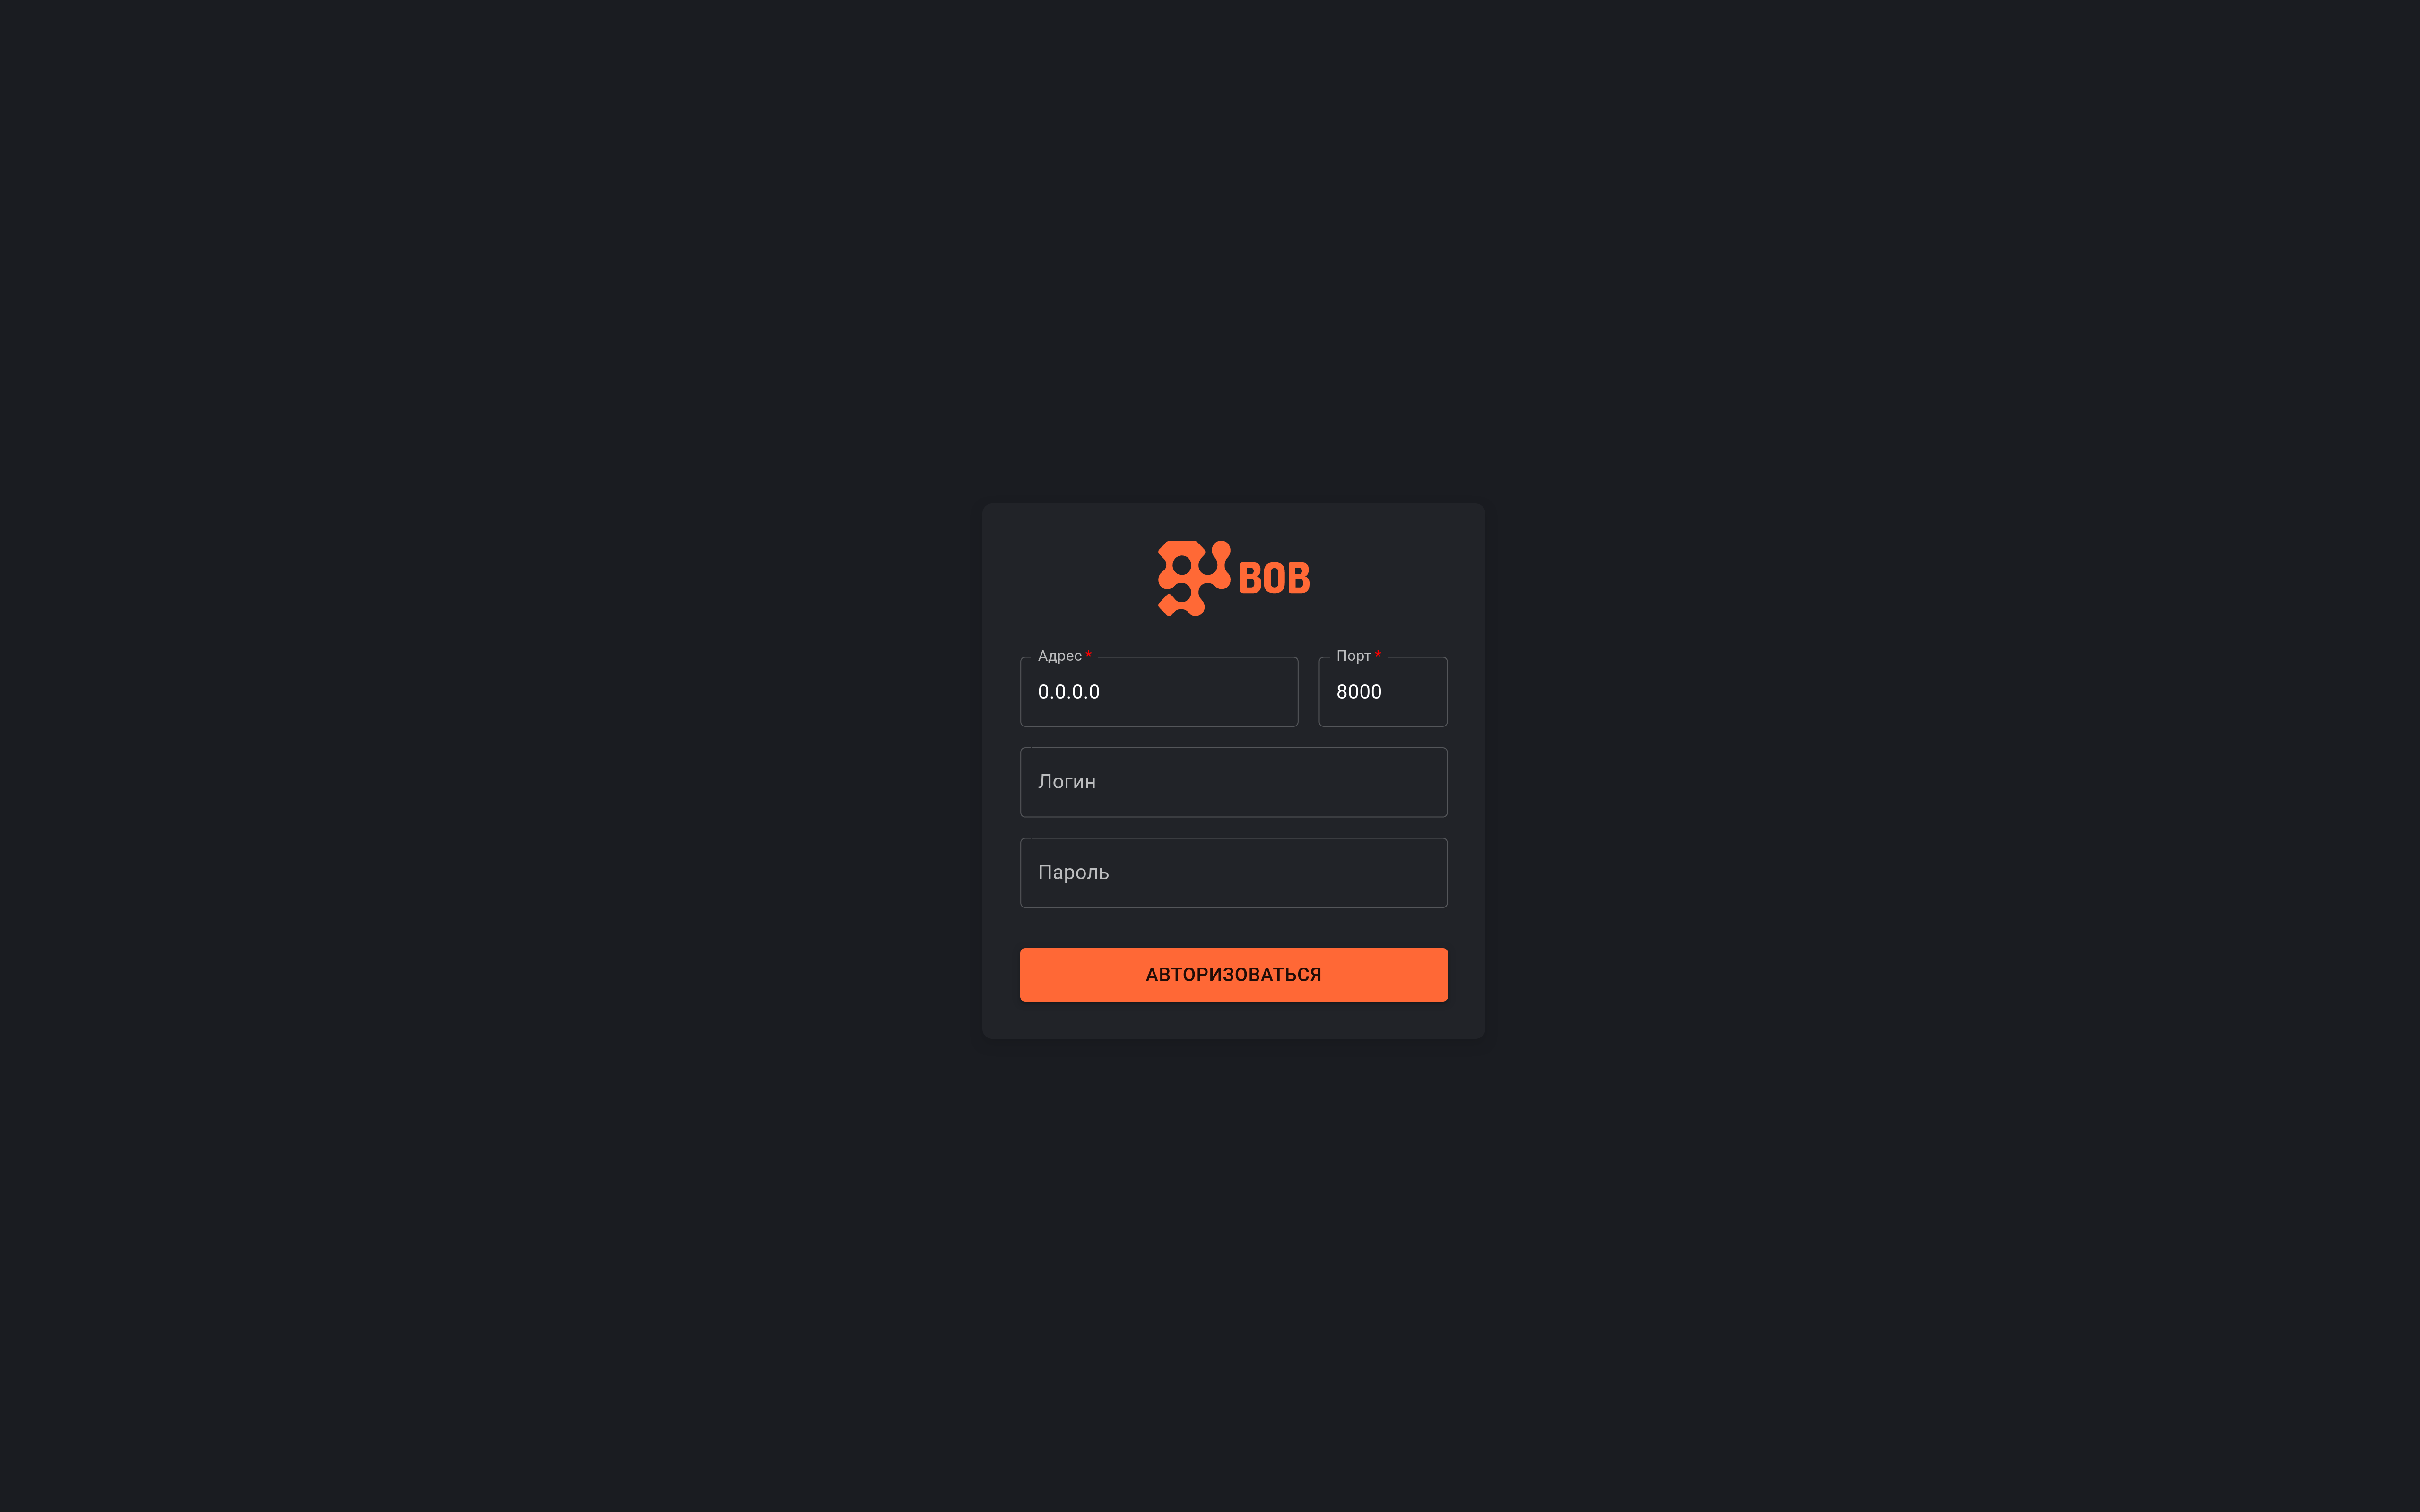
\includegraphics[width=0.95\textwidth]{inc/auth.png}
  \end{center}
  \caption{Страница авторизации}\label{fig:auth}
\end{figure}

\clearpage

На рисунке~\ref{fig:panel1} изображена страница мониторинга ресурсов кластера BOB, которая обновляется в реальном времени, обновление можно как отключить, так и установить частоту обновления информации:

\begin{figure}[!htbp]
  \begin{center}
    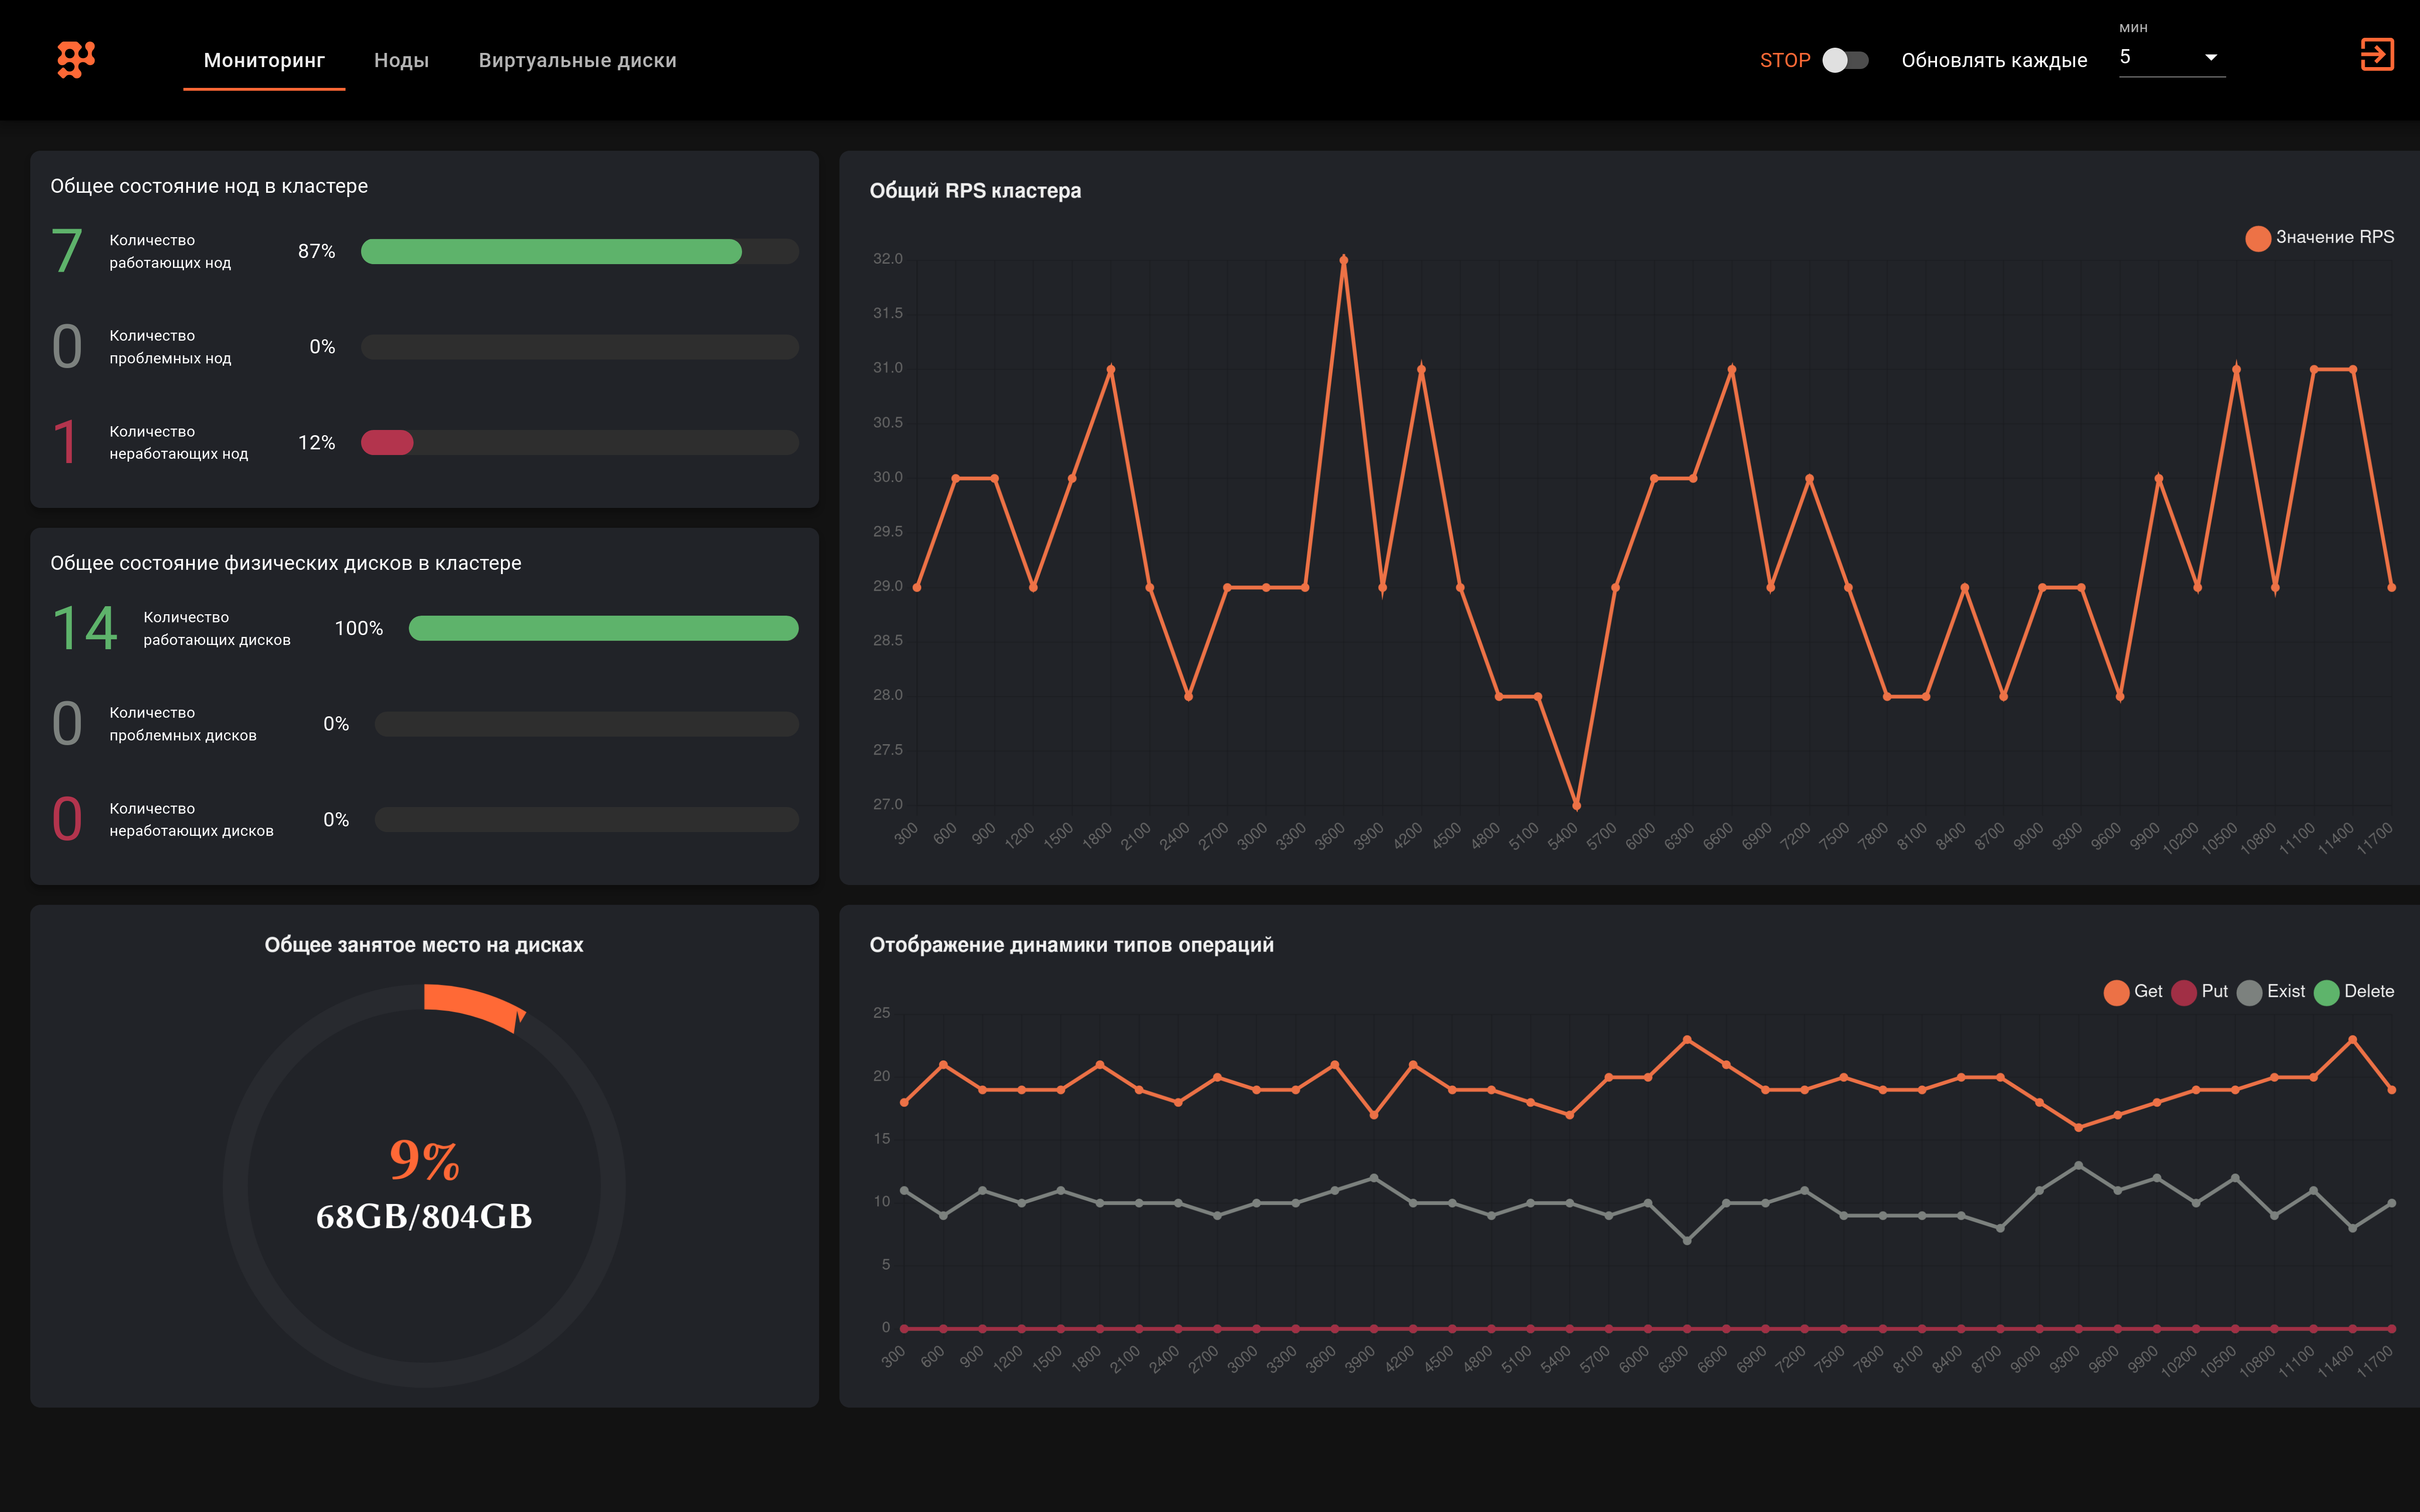
\includegraphics[width=0.95\textwidth]{inc/panel1.png}
  \end{center}
  \caption{Домашняя страница с основными параметрами кластера}\label{fig:panel1}
\end{figure}

\clearpage

На рисунке~\ref{fig:panel2} изображена информация по всем нодам:

\begin{figure}[!htbp]
  \begin{center}
    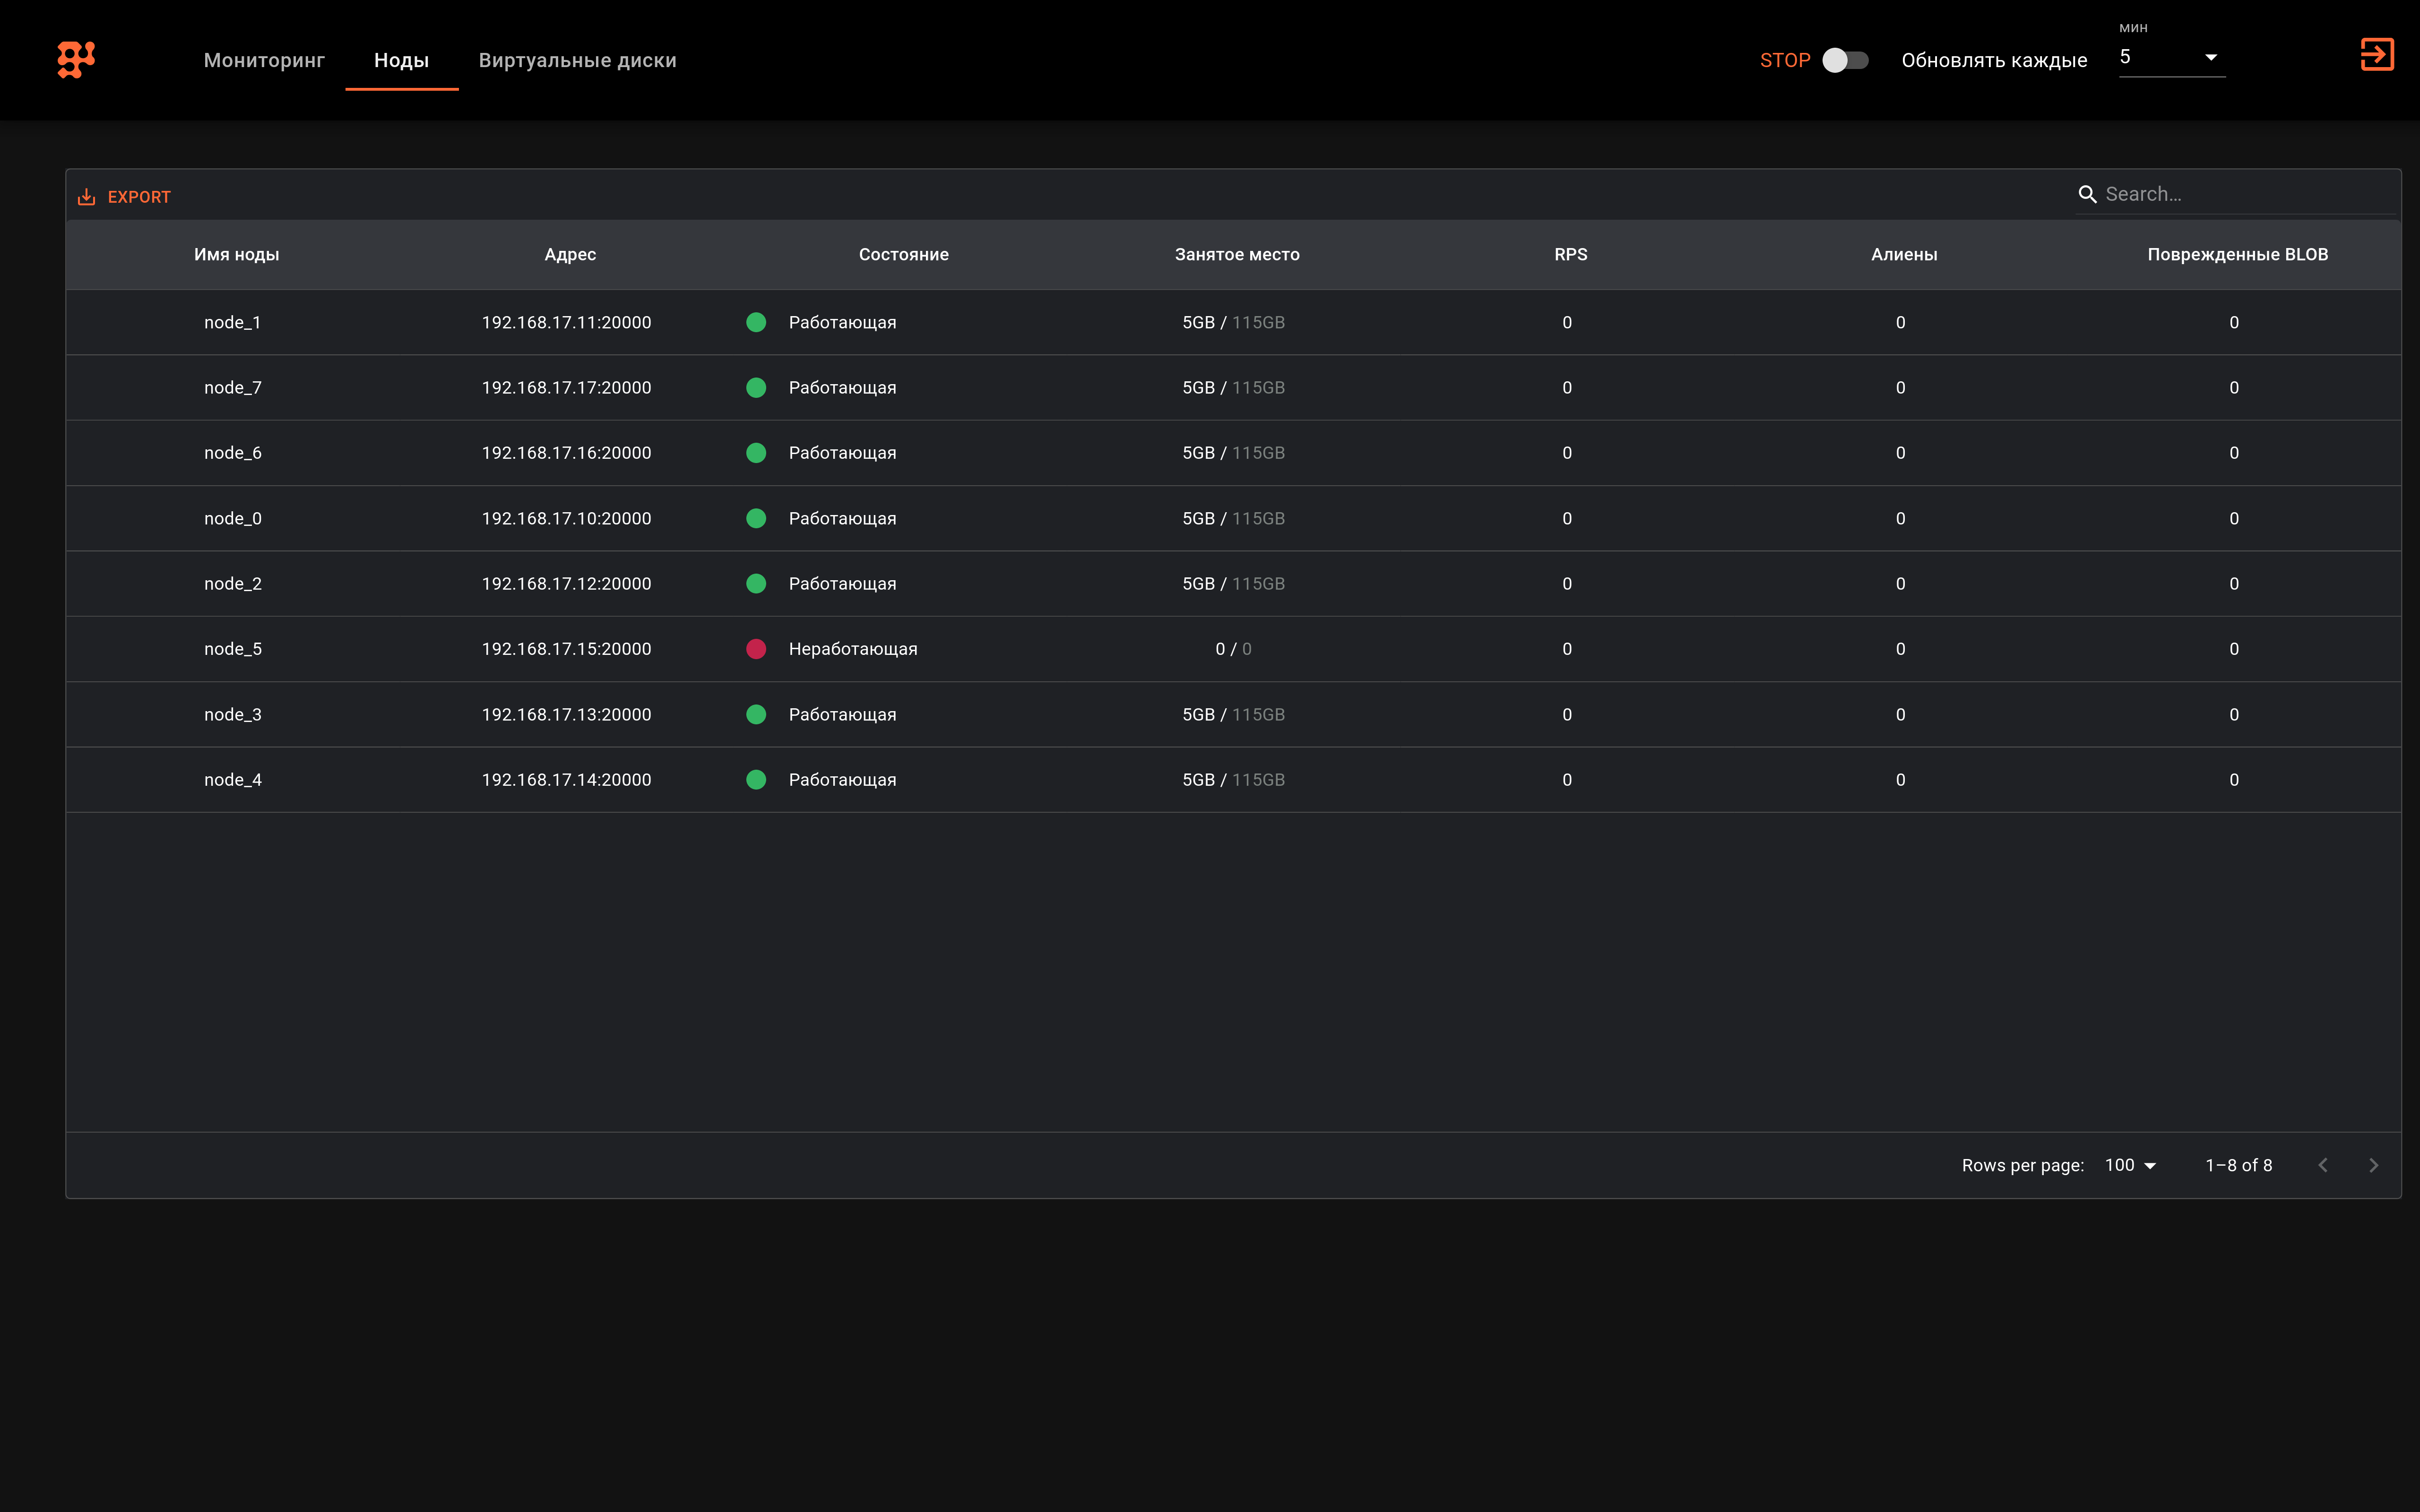
\includegraphics[width=0.95\textwidth]{inc/panel2.png}
  \end{center}
  \caption{Страница с нодами}\label{fig:panel2}
\end{figure}

\clearpage

На рисунке~\ref{fig:detailed_panel} изображена детальная информация по выбранной ноде из
списка предоставленного на рисунке~\ref{fig:panel2}:

\begin{figure}[!htbp]
  \begin{center}
    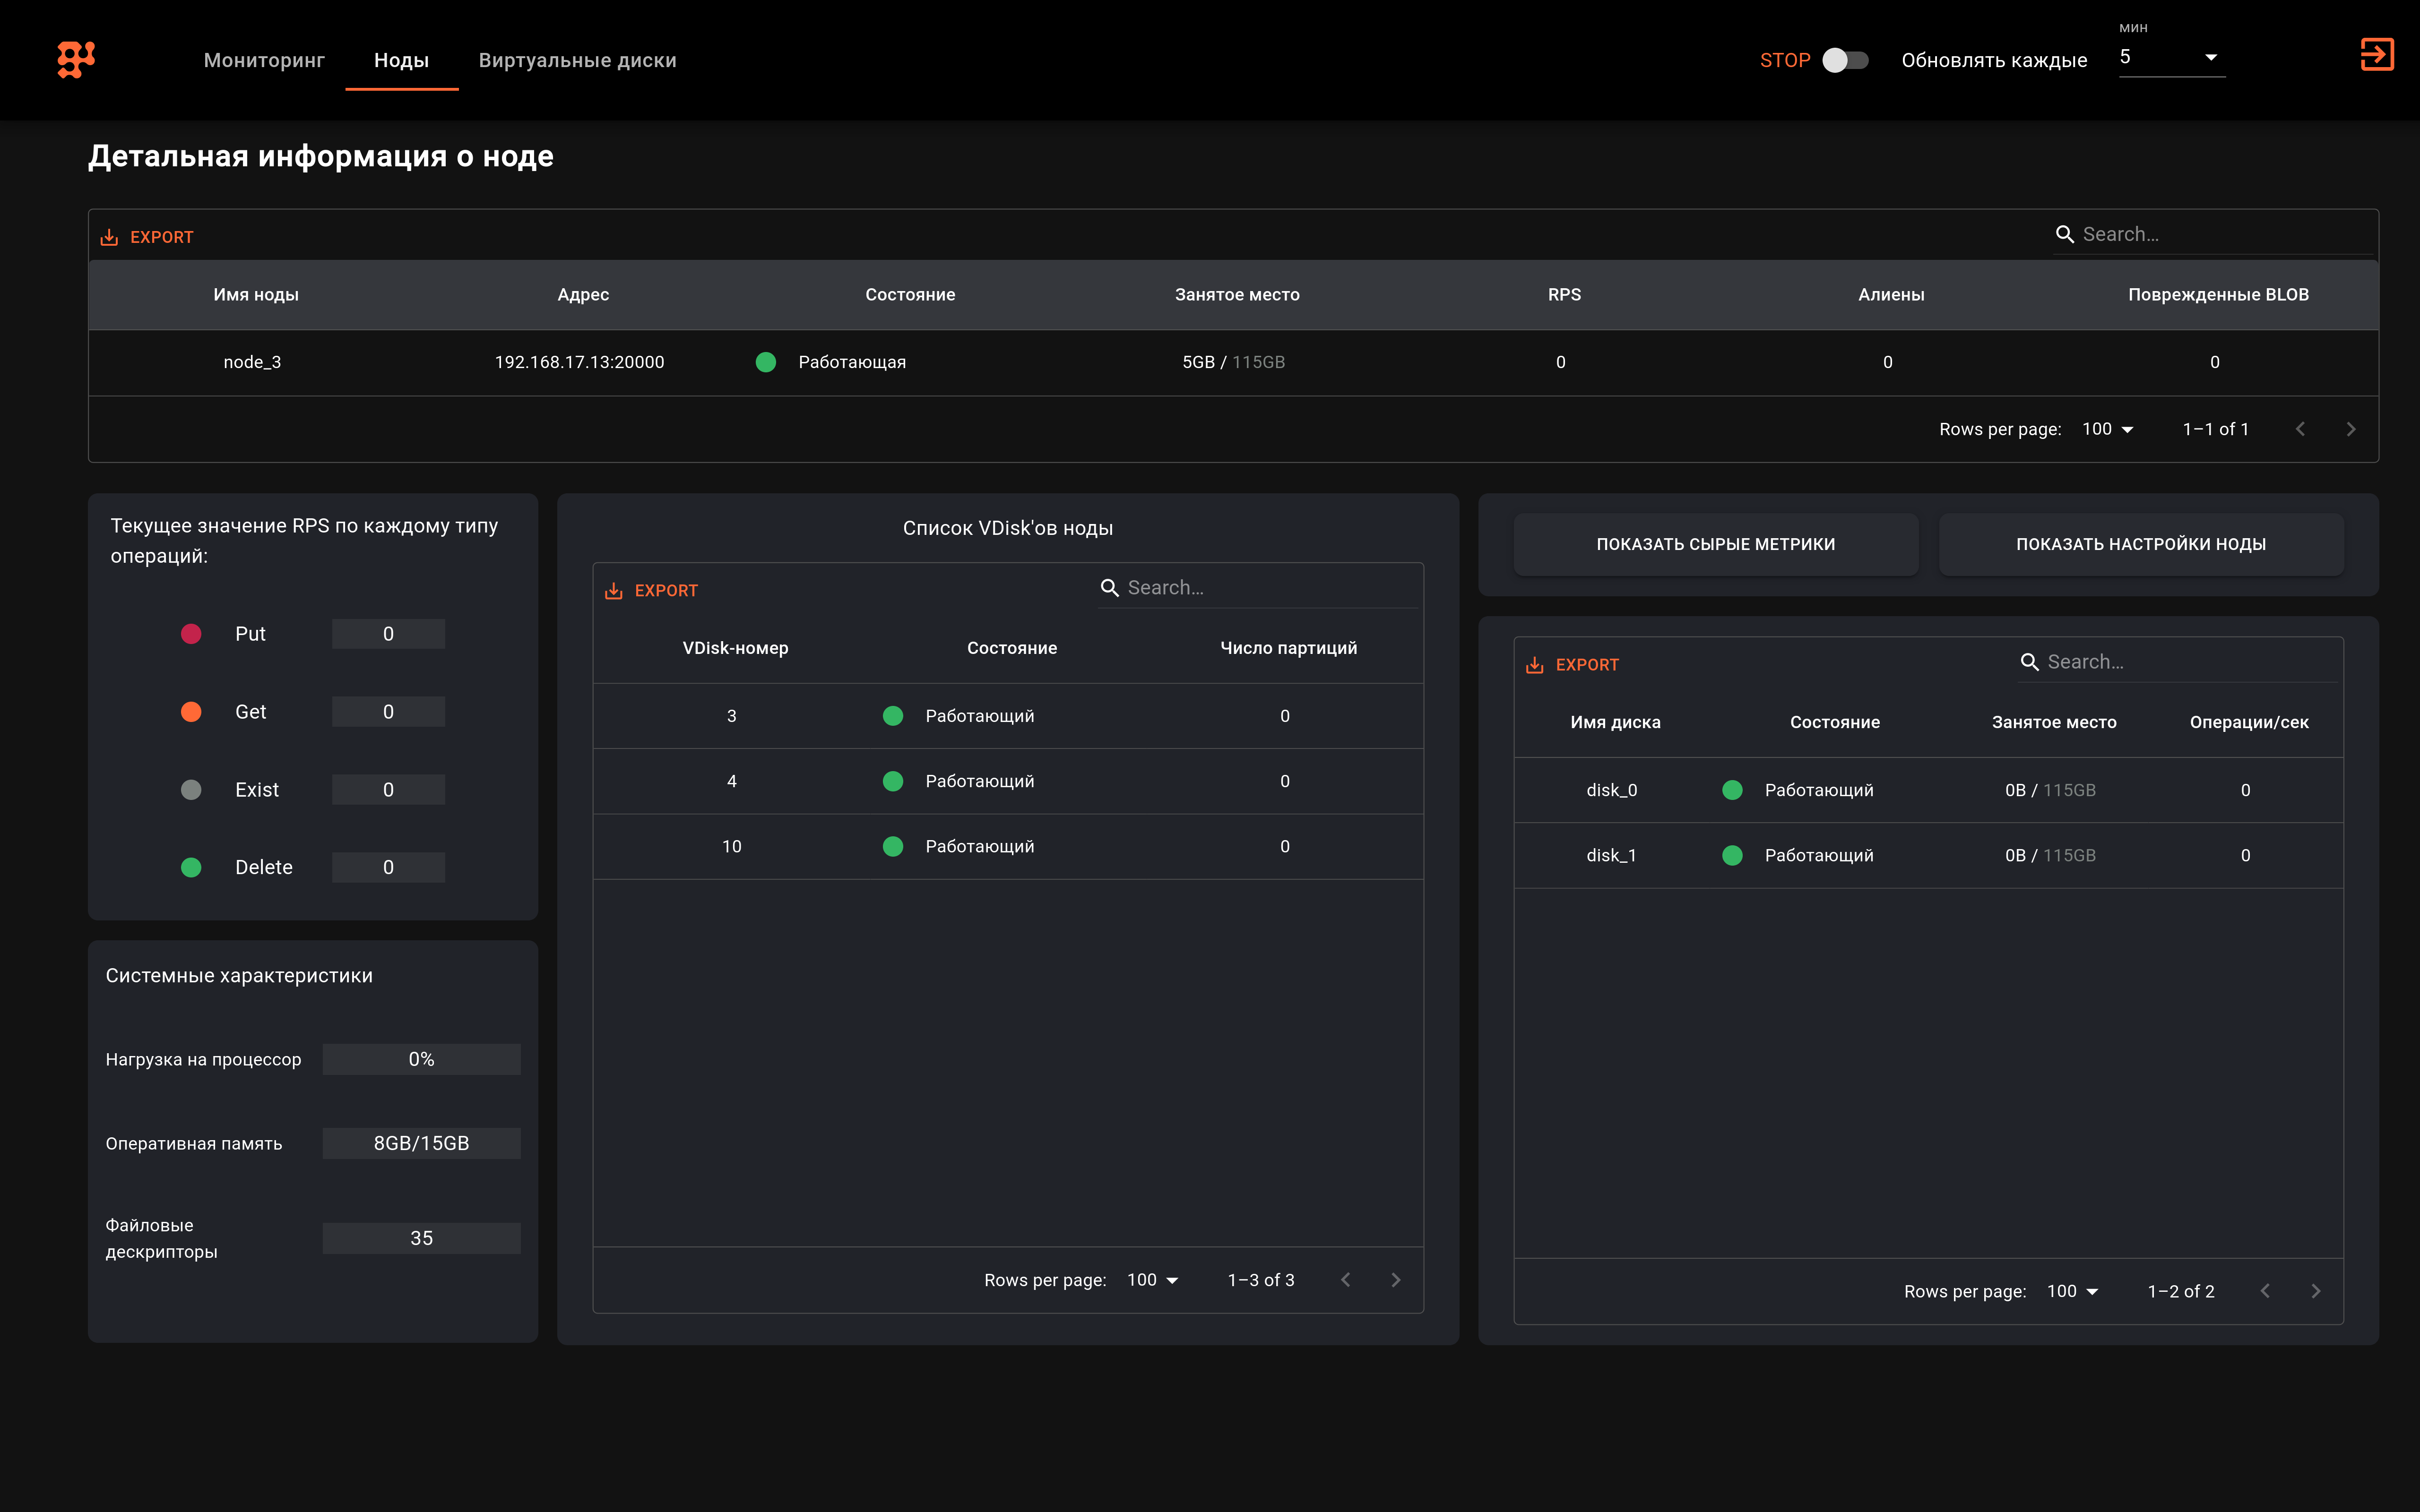
\includegraphics[width=0.95\textwidth]{inc/detailed_panel.png}
  \end{center}
  \caption{Страница с подробной информацией о ноде}\label{fig:detailed_panel}
\end{figure}

\clearpage

На рисунке~\ref{fig:panel3} изображена информация по всем виртуальным дискам:

\begin{figure}[!htbp]
  \begin{center}
    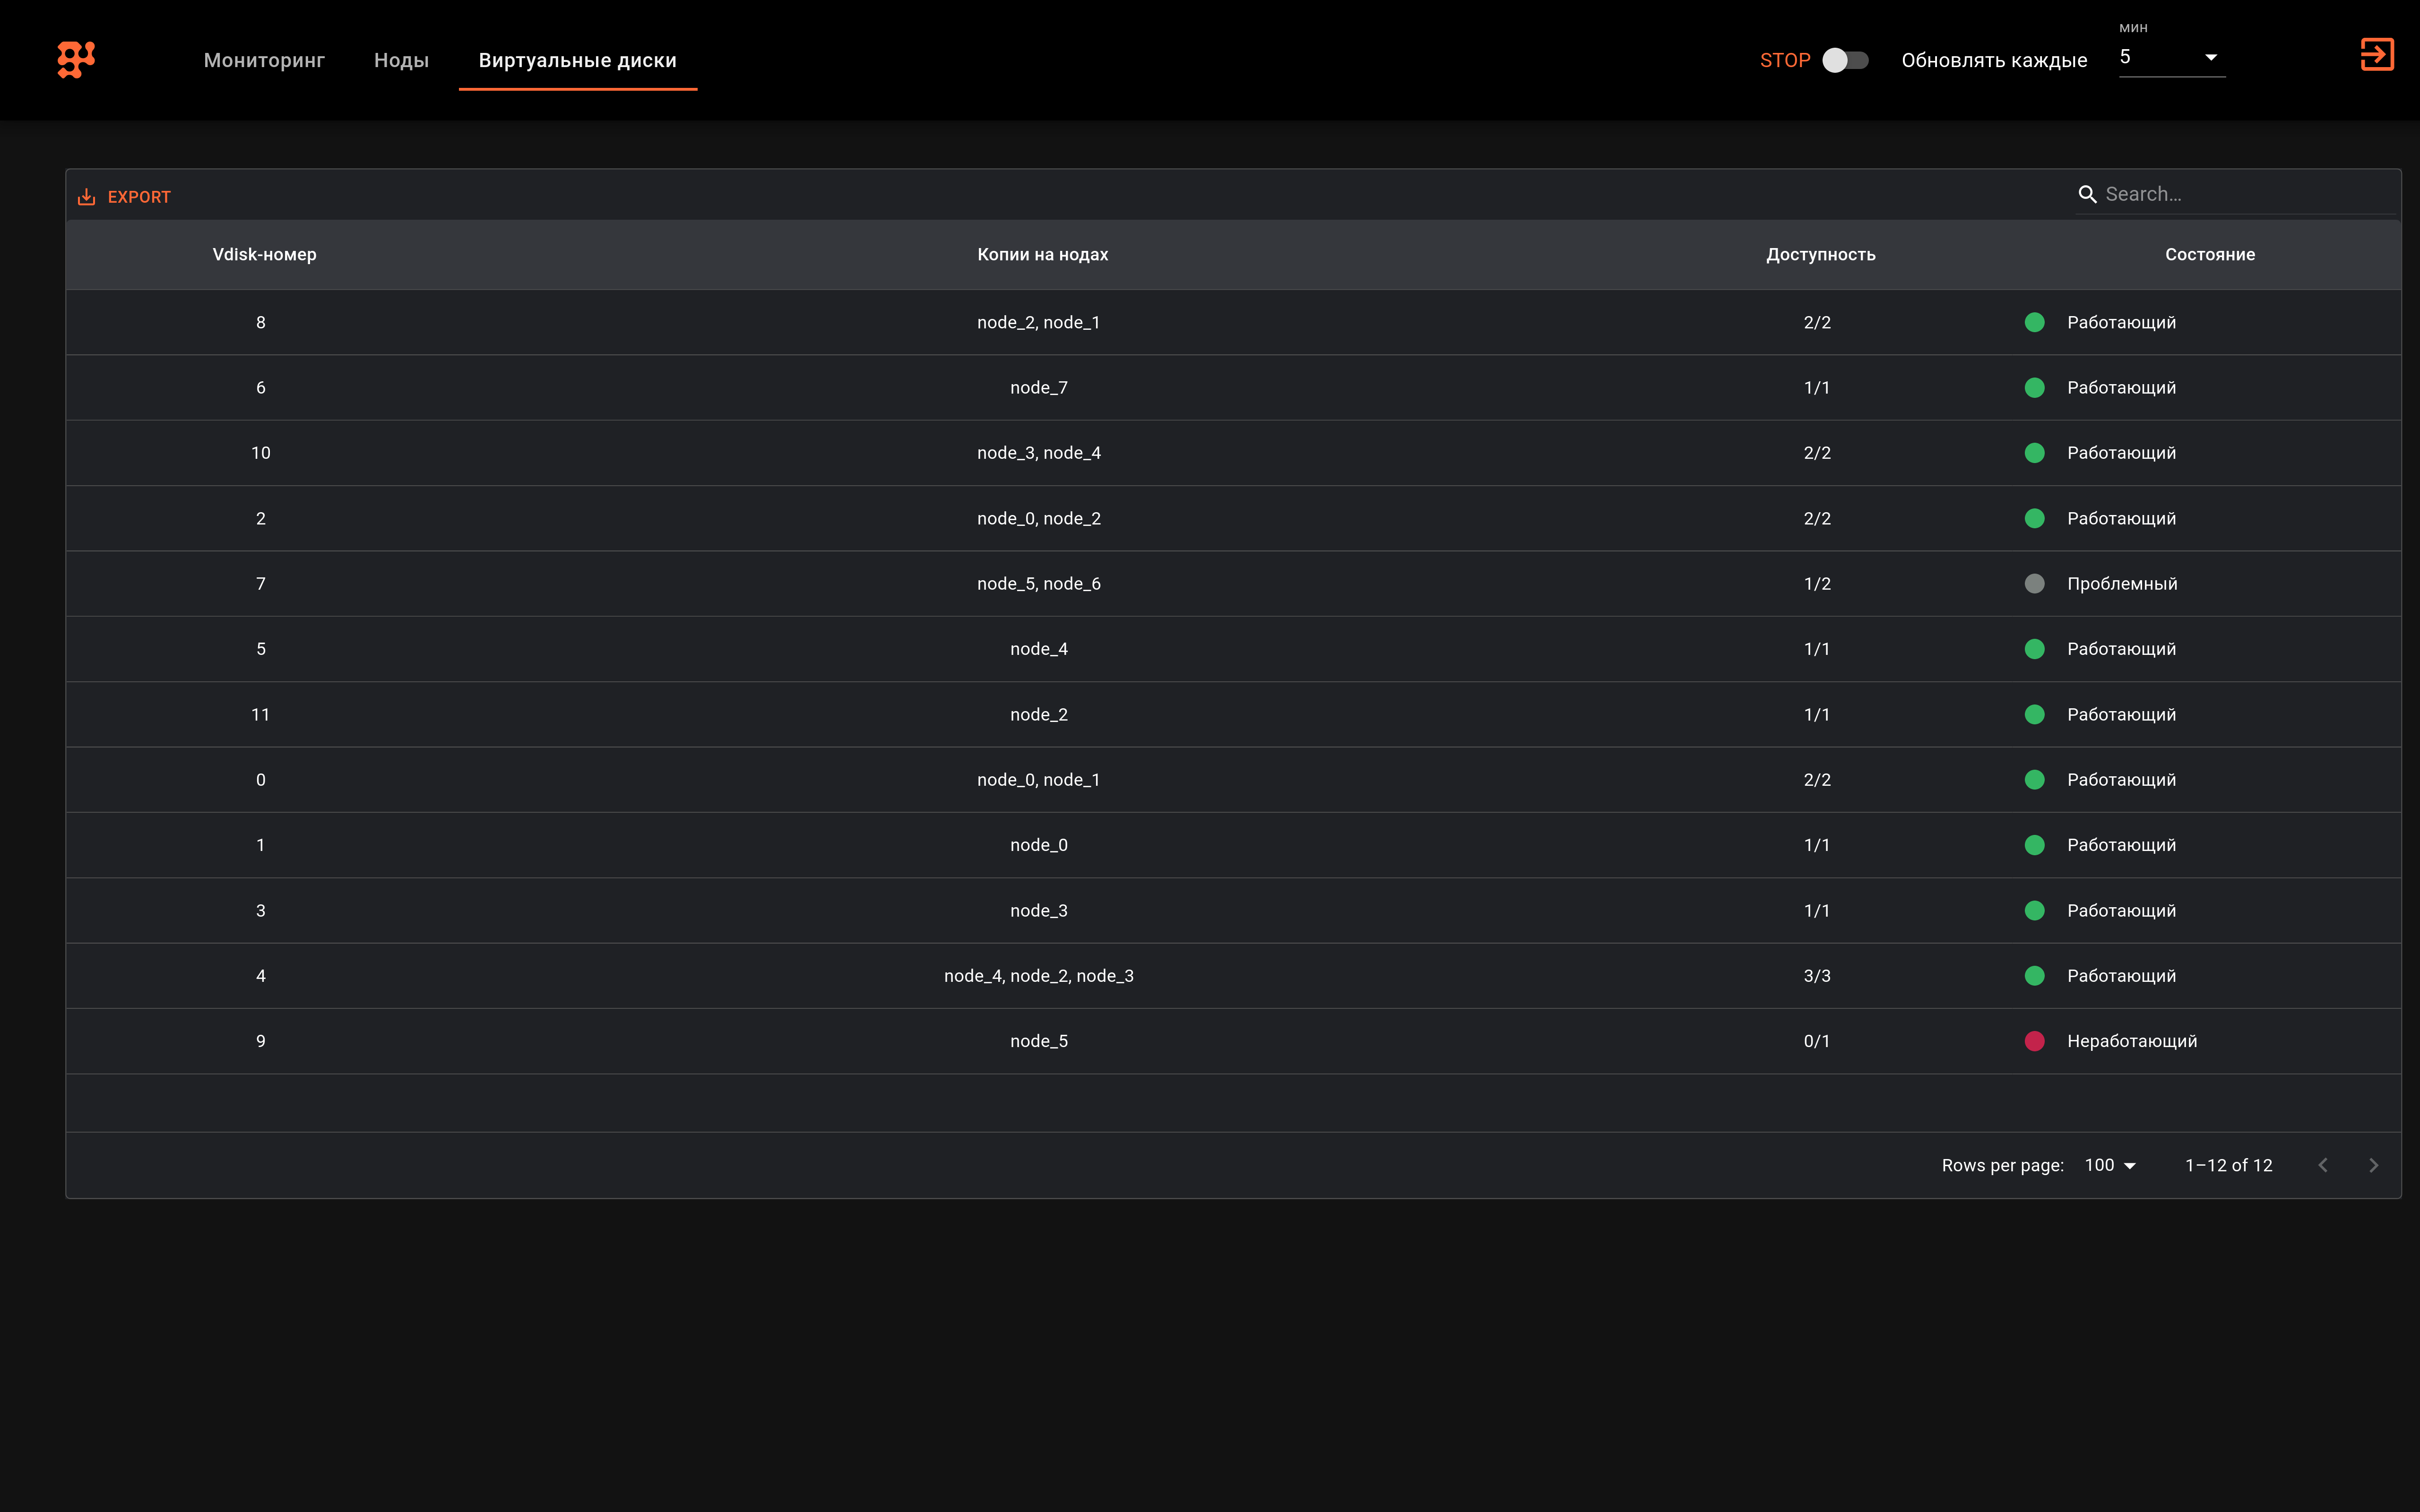
\includegraphics[width=0.95\textwidth]{inc/panel3.png}
  \end{center}
  \caption{Cтраница с раскладкой виртуальных дисков}\label{fig:panel3}
\end{figure}

\clearpage

\specsection{ЗАКЛЮЧЕНИЕ}

В ходе производственной практики были приобретены навыки в разработке веб-приложений и open source-проектов, а также было успешно разработано веб-приложение, предназначенное для эффективной работы с настройкой и управлением кластером BOB. 

Также были выполнены следующие индивдуальные задачи:
\begin{enumerate}
	\item получить навыки командной работы;
	\item спроектировать и разработать клиент для взаимодействия с API~\cite{api} Боба;
	\item спроектировать собственный API~\cite{api};
	\item разработать серверную часть веб-приложения, интегрируя в него ранее разработанный клиент и API~\cite{api};
	\item провести тестирование итогового Web-приложения.
\end{enumerate}

\clearpage

\specsection{СПИСОК ИСПОЛЬЗОВАННЫХ ИСТОЧНИКОВ}

\begingroup
\renewcommand{\section}[2]{}
\bibliographystyle{utf8gost705u}
\bibliography{bibliography}   
\endgroup

\end{document}
